\documentclass{beamer}
\usepackage{amssymb} % Therefore symbol
\usepackage{hyperref} % URLs
\title[Critical Thinking 6]{Critical Thinking \\Evaluating risk (Term 2)}
%\subtitle[short]{full}
\author{Andy J. Wills}
\institute[Plymouth University]{School of Psychology\\Plymouth University, U.K.}
\titlegraphic{
\includegraphics[width=.2\textwidth]{plym_logo.png}}


\begin{document}

\frame{\titlepage}

\begin{frame}{Revision}
\end{frame}

\begin{frame}{Probability}
\begin{itemize}
\item Probability (by the simplest objective definition) is that property which allows us to calculate the frequency of an event in a very long run of events.

\centerline{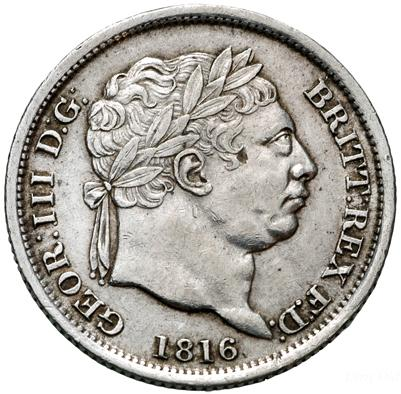
\includegraphics[width=0.2\textwidth]{coin.jpg}}
\item Fair coin 
\begin{itemize}
	\item $P(heads) = 0.5, P(tails) = 0.5$
	\item Flip a fair coin 1000 times, you get close to 500 heads.
	\item The more times you flip the more $heads/flips$ tends towards 0.5.
\end{itemize}
\end{itemize}
\end{frame}

\begin{frame}{Conditional probability}
\begin{itemize}
\item Smokers have lower life expectancy
\item $P(DeathBeforeSixty|smoker) = 0.2 $ 
\item $P(DeathBeforeSixty|nonsmoker) = 0.1 $
\end{itemize}
\end{frame}

\begin{frame}{Odds ratio}
\begin{itemize}
\item $P(DeathBeforeSixty|smoker) = 0.2 $ 
\item $P(DeathBeforeSixty|nonsmoker) = 0.1 $ 
\item Odds ratio, $OR = 0.2 / 0.1 $
\item $OR = 2$
\item Smoking doubles the risk of dying before sixty. 
\end{itemize}
\end{frame}

\begin{frame}{Conditional Probability and Randomness}
\begin{itemize}
\item Probability of some event, given that some other event is known to have occurred.
\item $P(heads_{t}|heads_{t-1}) = 0.5$
\item $P(heads_{t}|tails_{t-1}) = 0.5$
\item Events are \textbf{independent} if the conditional probabilities are equal to the unconditional probabilities (as close to an adequate definition of ``random'' as you're ever likely to get).
\item Coin flips, roulette wheels, etc. are demonstrably independent. 
\end{itemize}
\end{frame}

\begin{frame}{Gamblers' fallacy}
\centerline{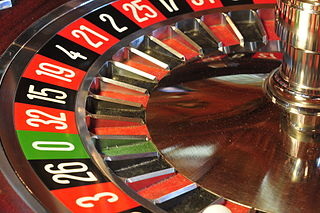
\includegraphics[width=0.4\textwidth]{roulette.jpg}}
\begin{itemize}
\item Red Red Black Red Black Black Black Black 
\item Bet ``red'', bet ``black'', or doesn't matter?
\item Common answer: ``bet red''
\item Rational answers
	\begin{itemize}
		\item If the wheel is known to be unbiased, $P(red) = P(black)$, and it doesn't matter.
		\item From the sample above estimates are that $P(red) < P(black)$, so  bet black.
	\end{itemize}
\end{itemize}
\end{frame}

\begin{frame}{Hot hand fallacy}
\begin{itemize}
\item Player A: Score Score Miss Miss
\item Player B: Miss Miss Score Score
\item A, B, or doesn't matter?
\item Common answer: ``Pass to B'' - Hot Hand fallacy
\item Gilovich, Vallone \& Tversky (1985) - Shots in basketball are independent.
\item Rational answer: Doesn't matter
\item Things to note:
	\begin{itemize}
	\item Basketball experts and players exhibit a hot hand fallacy
	\item Hot Hand and Gamblers' Fallacy are \textbf{opposite} beliefs about independent events. What drives this?
	\end{itemize}
\end{itemize}
\end{frame}

\begin{frame}{Dice game}
\end{frame}

% Regression to the mean

\begin{frame}{Regression to the mean}
\begin{itemize}
\item For \textbf{independent} events, an extreme event at time 1 is likely to be followed by a less extreme event at time 2.
\item This is simply because extreme events are less likely than non-extreme events.
\item Regression to the mean is widely neglected:
\begin{itemize}
\item Evaluation of the efficacy of school inspection programmes, prisoner rehabilitation, treatments for depression...
\item Disappointing post-transfer performance in footballers.
\item Disappointing sequels to great films, books, etc.
\item Why we prefer punishment over reward, even in situations where reward is more effective than punishment.
\end{itemize}
\end{itemize}
\end{frame}

\begin{frame}{GAME SHOW!}
\centerline{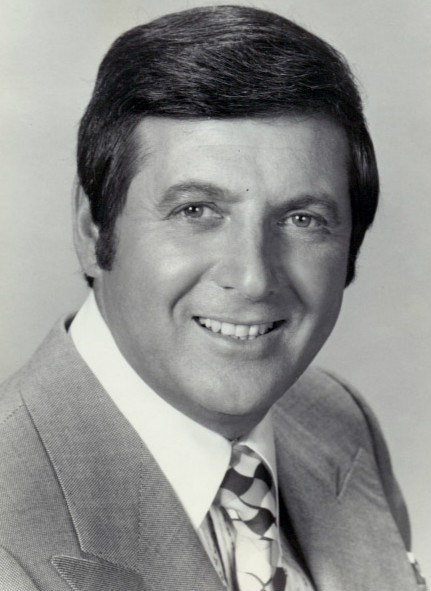
\includegraphics[width=0.3\textwidth]{montyphoto.jpg}}
\centerline{``Let's Make A Deal''}
\centerline{with your host, Monty Hall.}
\end{frame}

\begin{frame}{Monty Hall problem}
\centerline{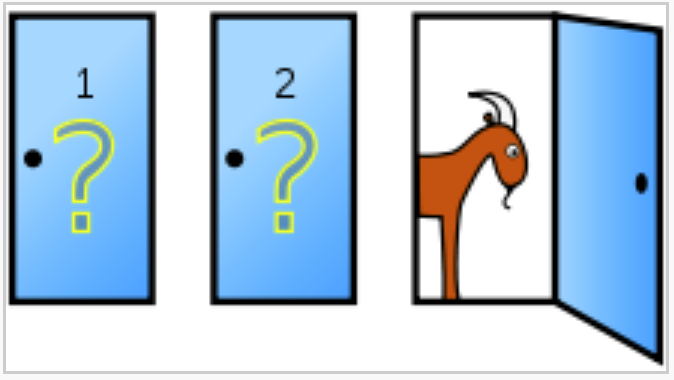
\includegraphics[width=0.5\textwidth]{montyhall.png}}
\begin{itemize}

\item Suppose you're on a game show, and you're given the choice of three doors: Behind one door is a car; behind the others, goats. You want to win the car. You pick a door, say No. 1, and the host, who knows what's behind the doors, opens another door, say No. 3, which has a goat. He then says to you, ``Do you want to pick door No. 2?'' Is it to your advantage to switch your choice? (vos Savant, 1990).
\begin{itemize}
\item Better to switch?
\item Better to stick?
\item Doesn't matter, stick or switch equally likely to win?
\end{itemize}
\end{itemize}
\end{frame}

\begin{frame}{Working out the Monty Hall problem}
\begin{itemize}
\item The host is not going to open the door with the car behind it.
\item On two-thirds of occasions, your first choice will be a goat.
\begin{itemize}
\item The host will then reveal the other goat.
\item So, the car is behind the other door.
\item If you switch, you will win the car
\end{itemize}
\item On one-third of occasions, your first choice will be the car.
\begin{itemize}
\item If you switch, you will not win the car.
\end{itemize}
\item So, on two-thirds of occasions, switching will win the car.
\item You should always switch.
\end{itemize}
\end{frame}

\begin{frame}{Linda}
\begin{itemize}
\item Linda is 31 years old, single, outspoken, and very bright. She majored in philosophy. As a student, she was deeply concerned with issues of discrimination and social justice, and also participated in anti-nuclear demonstrations.
\item Which is more probable?
\begin{enumerate}
\item Linda is a bank teller.
\item Linda is a feminist bank teller.
\end{enumerate}
\end{itemize}
\end{frame}

\begin{frame}{Conjunction fallacy}
\begin{itemize}
\item Which is more probable?
\begin{enumerate}
\item Linda is a bank teller
\item Linda is a bank teller and is active in the feminist movement.
\end{enumerate}
\item The probability of two events both happening can NEVER be higher than the probability of just one happening. 
\end{itemize}
\end{frame}

\begin{frame}{The conjunction rule}
The probability of two \emph{independent} events both occurring is the product of their individual probabilities.
\begin{itemize}
\item $P(heads_{time 1}) = 0.5$
\item $P(heads_{time 2}) = 0.5$
\item $P(heads_{times 1 and 2}) = P(heads_{time 1}) \times P(heads_{time 2}) = 0.5 \times 0.5 = 0.25$
\item $P(teller) = .05, P(feminist) = .95$
\item $P(teller + feminist) = .05 \times .95 = .0475$
\item $P(teller + feminist) < P(feminist)$
\end{itemize}
\end{frame}

\begin{frame}{Sally Clark}
\centerline{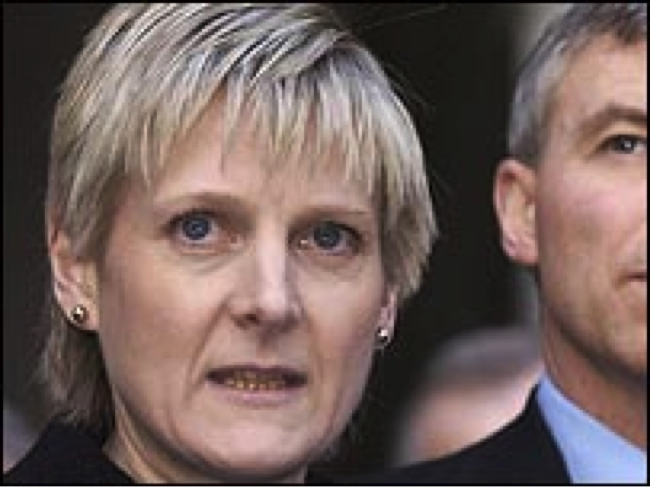
\includegraphics[width=0.5\textwidth]{sallyclark.png}}
\begin{itemize}
\item Solicitor; born 1964.
\item Christopher died at 11 weeks.
\item One year later, Harry died at 8 weeks.
\item Little to no forensic evidence.
\item No evidence she had been a violent or uncaring parent.
\end{itemize}
\end{frame}

\begin{frame}{Roy Meadows}
\centerline{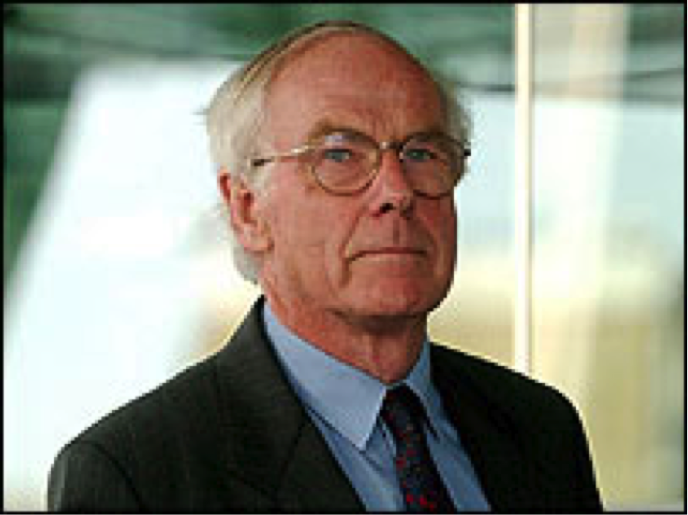
\includegraphics[width=0.5\textwidth]{roymeadows.png}}
\begin{itemize}
\item Sally convicted of murder, spent three years in prison
\item Central to conviction was evidence of expert witness Prof. Roy Meadows:
\begin{itemize}
\item Probability of two cot deaths in the same family was 1 in 73 million
\item Less than once a century in the UK.
\end{itemize}
\item Released on appeal, partly because Prof. Meadows's \textbf{probabilistic inference} was demonstrably wrong.
\end{itemize}
\end{frame}

% Sally Clark; wrong and right statistics. (10 minutes)

\begin{frame}{Roy Meadows - expert witness}
\begin{itemize}
\item Chances of a randomly chosen baby dying of cot death are 1 in 1303, $p = .0008$
\item If the family is affluent, and the mother is over 26, then the chances are even lower; 1 in 8500, $p = .0001$
\item Through the multiplicative law, the probability of two cot deaths in the same family is $ .0001 \times .0001 = 1 \times 10^{-8}$
\item 1 in 73 million
\item Less than once a century in the UK.
\item The idea that these deaths were by natural causes can be ruled out beyond \emph{reasonable doubt}.
\end{itemize}
\end{frame}

\begin{frame}{Roy Meadows - expert witness}
\begin{itemize}
\item Chances of a randomly chosen baby dying of cot death are 1 in 1303, $p = .0008$
\item If the family is affluent, and the mother is over 26, then the chances are even lower; 1 in 8500, $p = .0001$
\item Through the \textbf{multiplicative law}, the probability of two cot deaths in the same family is $ .0001 \times .0001 = 1 \times 10^{-8}$ ... \textbf{COT DEATHS WITHIN THE SAME FAMILY ARE HIGHLY UNLIKELY TO BE INDEPENDENT EVENTS}.
\item 1 in 73 million
\item Less than once a century in the UK.
\item The idea that these deaths were by natural causes can be ruled out beyond \emph{reasonable doubt}.
\end{itemize}
\end{frame}

\begin{frame}{Freak weather}
	\begin{itemize} 
		\item Hurricanes are a 1 in 100 year weather event in Plymouth. What's the probability there will be a hurricane in Plymouth in the next 100 years? (Ignore climate change; assume independence).
		\item 1, .9, .6
	\end{itemize}
\end{frame}

\begin{frame}{High-school maths}
\begin{itemize}
\item $3 \times 3 = 3^2 $
\item $4 \times 4 \times 4 = 4^3$
\item And so on, e.g. $0.5^8 = .5 \times .5 \times .5 \times .5 \times .5 \times .5 \times .5 \times .5 $
\item Any number less than one (all probabilities) -- the answer gets small quite quickly
\item $.99^2 = .98$
\item $.99^{10} = .90$
\item $.99^{20} = .82$
\item $.99^{50} = .61$
\item $.99^{100} = .37$
\end{itemize}
\end{frame}

\begin{frame}{Hurricane example}
	\begin{itemize} 
		\item In each of 100 years, there is a .01 chance of a hurricane.
		\item So, the chance of no hurricane in a given year is .99 (there's either a hurricane or there isn't and these two probabilities must add to 1).
		\item For there to be no hurricane in the next 100 years, there has to be no hurricane in each of those 100 years.	
		\item Under the conjunction rule, therefore, $p = .99^{100} = .37$	
		\item So, the chance of a 1 in 100 year weather event occurring in the next 100 years is $1-.37=.63$
	\end{itemize}
\end{frame}

\begin{frame}{Shared birthdays}
	\begin{itemize} 
		\item In a class of 30 children, what's the probability that there is a shared birthday in the class? (Assume independence, and equiprobability of birth date).
		\item More likely there is, or more likely there is not?
	\end{itemize}
\end{frame}

\begin{frame}{More high-school maths}
\begin{itemize}
\item Number of pairs: $n(n-1)/2$
\item This gets very large quite quickly.
\item Pairs in a group of 2: $2(1)/2 = 1$
\item Pairs in a group of 5: $5(4)/2 = 10$
\item Pairs in a group of 10: $10(9)/2 = 45$
\item Pairs in a group of 20: $20(19)/2 = 190$
\item Pairs of children in a class of 30: $30(29)/2 = 435$
\item Pairs in Year 1 psychology, approx: $300(299)/2 = 44850$
\end{itemize}
\end{frame}

\begin{frame}{Birthday example}
	\begin{itemize} 
		\item 365 days in the year (ignore Feb 29th).
		\item So, the chance of one pair of kids sharing a birthday is $1/365 = .003$
		\item Thus, chance of not sharing is .997
		\item If no pair of kids share a birthday, then there is no shared birthday in the class.
		\item How many pairs in the class?
		\item $n(n-1)/2 = 30 \times 29/2 = 435$.	
		\item Under conjunction rule, $p = .997^{435} = .17$
		\item Thus, probability of a shared birthday is 1-.17 = .83	
	\end{itemize}
\end{frame}

\begin{frame}{Summary}
\begin{itemize}
\item Regression to the mean
\item The Monty Hall problem
\item Conjunction rule (Linda)
\item Events are not always independent (Sally Clarke)
\item If a lot of things all have to happen, this is quite unlikely, even if each event is individually very likely (avoiding hurricanes for 100 years; all non-shared birthdays in a class of 30).
\item The number of pairs in a large group is much bigger than you think it is. This can often lead us to make incorrect predictions about large groups. 
\end{itemize}
\end{frame}

% Reading
\begin{frame}{Further Reading}
Helpful background, only lecture content on these topics is examinable).
\begin{itemize}
\item Paulos (1988/2000). \emph{Innumeracy}. Penguin.
\item  \url{http://en.wikipedia.org/wiki/Conjunction_fallacy}
\item  \url{http://en.wikipedia.org/wiki/Sally_Clark}
\item  \url{http://en.wikipedia.org/wiki/Probability}
\end{itemize}
\end{frame}



\end{document}
